% Build:  pdflatex hypothesis_bandit.tex   (twice, for references)
\documentclass[11pt]{article}
\usepackage[margin=1in]{geometry}
\usepackage{amsmath,amssymb}
\usepackage[ruled,vlined,linesnumbered]{algorithm2e}
\usepackage{booktabs}
\usepackage{tikz}
\usepackage{xcolor}
\usepackage[colorlinks=true,linkcolor=black,citecolor=black,urlcolor=blue]{hyperref}
\usetikzlibrary{arrows.meta,positioning,fit,backgrounds}

\definecolor{ink}{HTML}{1F2328}
\definecolor{sub}{HTML}{57606A}
\definecolor{edge}{HTML}{D0D7DE}
\definecolor{panel}{HTML}{F6F8FA}
\definecolor{hypcol}{HTML}{8250DF}
\definecolor{codecol}{HTML}{0969DA}
\definecolor{good}{HTML}{1A7F37}
\definecolor{bad}{HTML}{CF222E}

\title{\textbf{HypothesisBandit}\\[2mm]
\large Hypothesis-guided adaptive co-evolution for program search}
\author{Pantheon-Evolve \\ \small\texttt{pantheon.evolution.methods.HypothesisBandit}}
\date{September 2026}

\begin{document}
\maketitle

\begin{abstract}
\noindent Most LLM-driven code evolution searches over \emph{programs}: mutate, measure, keep the
winners. Attribution is then impossible --- a mutation touches several things at once, the score
moves, and the run learns nothing transferable about \emph{why}. HypothesisBandit searches over
\emph{stated claims about the program} and treats programs as evidence for those claims. Two
coupled populations (hypotheses $H$, programs $P$) are linked by an anchor relation; every
implementation is edit-shaped and touches exactly one named component, which makes observational
credit assignment well defined; and a bandit over measured evidence --- deliberately with no LLM
judge --- allocates the remaining budget. This document specifies the algorithm, states the
empirical reasons for each design choice, and reports what it does and does not buy.
\end{abstract}

\section{The two populations}

\begin{center}
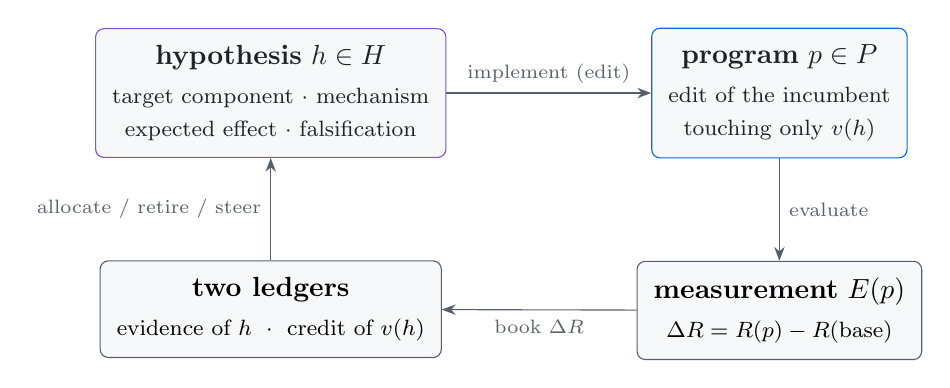
\begin{tikzpicture}[
  node distance=6mm,
  box/.style={rounded corners=3pt, draw=edge, fill=panel, inner sep=6pt, align=center},
  hyp/.style={box, draw=hypcol, text=ink, minimum width=44mm},
  prog/.style={box, draw=codecol, text=ink, minimum width=30mm},
  ar/.style={-{Stealth[length=5pt]}, draw=sub},
]
\node[hyp] (h) {\textbf{hypothesis} $h \in H$\\[2pt]
  \footnotesize target component $\cdot$ mechanism\\
  \footnotesize expected effect $\cdot$ falsification};
\node[prog, right=26mm of h] (p) {\textbf{program} $p \in P$\\[2pt]
  \footnotesize edit of the incumbent\\ \footnotesize touching only $v(h)$};
\node[box, below=13mm of p, draw=sub] (e) {\textbf{measurement} $E(p)$\\[2pt]
  \footnotesize $\Delta R = R(p) - R(\text{base})$};
\node[box, below=13mm of h, draw=sub] (l) {\textbf{two ledgers}\\[2pt]
  \footnotesize evidence of $h$ $\;\cdot\;$ credit of $v(h)$};
\draw[ar] (h) -- node[above,font=\scriptsize,text=sub]{implement (edit)} (p);
\draw[ar] (p) -- node[right,font=\scriptsize,text=sub]{evaluate} (e);
\draw[ar] (e) -- node[below,font=\scriptsize,text=sub]{book $\Delta R$} (l);
\draw[ar] (l) -- node[left,font=\scriptsize,text=sub]{allocate / retire / steer} (h);
\end{tikzpicture}
\end{center}

\noindent A program records its hypothesis as \texttt{anchor\_id} and the component it changed as
\texttt{meta["component"]}. The cycle $h \to p \to E(p) \to \text{ledgers} \to h'$ is the whole
method; everything below is how each arrow is implemented.

\section{Algorithm}

\begin{algorithm}[H]
\SetAlgoLined
\DontPrintSemicolon
\KwIn{seed program $p_0$, component vocabulary $V$, budget $B$}
\KwOut{best measured program}
$H \gets \emptyset$;\quad $G_h \gets \emptyset\ \forall h$ \tcp*{per-hypothesis $\Delta R$ list}
$C_v \gets \emptyset\ \forall v \in V$ \tcp*{per-component $\Delta R$ list}
\While{budget remains}{
  \eIf{$|\{h : \text{live}\}| < H_{\min}$ \textbf{or} draw says propose}{
    $v^\star \gets \arg\max_{v \in V} \big[ A(v) + \lambda\,\sigma_v \big]$
      \tcp*{highest-headroom component}
    $h \gets \textsc{ProposeHypothesis}(v^\star, \text{diagnostics})$\;
    \lIf{$\textsc{StructuralGate}(h)$}{$H \gets H \cup \{h\}$ \textbf{with} $G_h \gets \emptyset$}
  }{
    $h \gets \textsc{SoftmaxSample}\big(\{\text{live } h\},\ \text{priority},\ \tau\big)$\;
    $p \gets \textsc{EditImplement}(h, \textsc{BestCode}(h))$
      \tcp*{change only $v(h)$}
    \If{task has a cheap fidelity}{
      $r_{\text{low}} \gets E_{\text{low}}(p)$\;
      \lIf{$r_{\text{low}} < R^\star - \delta$}{\textbf{reject}; $\text{fails}_h {+}{=} 1$;
        \textbf{continue}}
    }
    $r \gets E_{\text{full}}(p)$;\quad $\Delta R \gets r - R(\text{base}(p))$\;
    $G_h \gets G_h \cup \{\Delta R\}$;\quad $C_{v(h)} \gets C_{v(h)} \cup \{\Delta R\}$
      \tcp*{one number, two ledgers}
    \If{$|G_h| \ge 2$ \textbf{and} $\overline{G_h} \le 0$ \textbf{or} $\text{fails}_h \ge 2$}{
      retire $h$ \tcp*{evidence, not opinion}
    }
  }
}
\caption{HypothesisBandit}
\end{algorithm}

\section{The controller}

\paragraph{Priority and sampling.} For a live hypothesis $h$ with $n = |G_h|$ measurements,
\[
  \mu_h = \frac{1}{n}\sum_{g \in G_h} g, \qquad
  \sigma_h = \frac{\sigma_0}{\sqrt{1+n}}, \qquad
  \text{nov}_h = \frac{1}{1+n},
\]
\[
  \boxed{\ \text{priority}(h) \;=\; \mu_h \;+\; \lambda\,\sigma_h \;+\; \eta\,\text{nov}_h\ }
  \qquad
  \Pr(h) \;=\; \frac{\exp(\text{priority}(h)/\tau)}{\sum_{h'} \exp(\text{priority}(h')/\tau)}
\]
with defaults $\lambda = 1.0$, $\eta = 0.5$, $\tau = 0.35$, $\sigma_0 = 0.05$. Untried hypotheses
are separated only by novelty, so the opening is near-uniform; as evidence accumulates $\mu$
dominates and the distribution concentrates.

\paragraph{Component credit.} With $\overline{\Delta R}$ the mean gain over all measurements,
\[
  A(v) \;=\; \mathbb{E}\big[\Delta R \mid v \text{ changed}\big] - \mathbb{E}\big[\Delta R\big]
  \;=\; \frac{1}{|C_v|}\sum_{g \in C_v} g \;-\; \overline{\Delta R},
\]
estimated observationally --- no counterfactual re-runs. The next proposal targets
$\arg\max_v [A(v) + \lambda \sigma_v]$, so components with high measured payoff \emph{or} no data
yet get the next hypothesis. This is what makes the search direction itself adaptive.

\paragraph{Why no LLM judge.} The controller scores hypotheses by measurement only. On AHC039 an
ablation over the judge's information content inverted the expected ordering:

\begin{center}
\begin{tabular}{lcc}
\toprule
judge used for idea selection & improving children & \\
\midrule
random         & 9\,/\,56 & best \\
constant       & 2\,/\,47 & \\
LLM opinion    & \textbf{0\,/\,39} & worst \\
\bottomrule
\end{tabular}
\end{center}

\noindent An LLM's opinion about which idea to build was worse than noise on this search, so the
method spends no budget acquiring it.

\section{Why implementations are edits}

The predecessor method (AnnealedIdeaCode) implemented an idea by \emph{rewriting} the program from
it. On a mature seed that wrecked $84\%$ of attempts: the rewrite discards tuned constants,
schedules and micro-optimisations that no one asked it to change. HypothesisBandit instead
instructs the coding agent:

\begin{quote}\itshape
``You are an expert algorithm engineer testing a specific hypothesis by EDITING an existing
program. Change only what the hypothesis targets; keep the rest of the program intact. Verify your
edit with the evaluator before submitting.''
\end{quote}

\noindent Two consequences: the incumbent's quality is preserved by construction, and because only
one component moved, $\Delta R$ can be attributed to it --- credit assignment is a \emph{result}
of the edit discipline, not a separate estimator.

\section{A real run, step by step}

AHC039 (\emph{Purse Seine Fishing}), seed = a 5th-place contest solution scoring $\approx 3703$
official points per case. Every row below is recorded state from \texttt{wave4/seed 0}.

\begin{center}
\begin{tabular}{llrl}
\toprule
event & hypothesis (component) & $\Delta R$/case & consequence \\
\midrule
propose $\times 4$ & --- & --- & opening archive, priority $=$ novelty \\
measure & seed from 3 best rects (\emph{init}) & $+16.4$ & promising \\
measure & retune cooling (\emph{params}) & $+9.0$ & promising \\
measure & fill rectangular bays (\emph{output}) & $-11.8$ & \\
measure & fill rectangular bays (\emph{output}) & $+3.2$ &
  \textbf{run's best program}, \emph{and} retired \\
measure & exact sweep rescorer (\emph{core}) & $-35.8$ & \\
measure & exact sweep rescorer (\emph{core}) & $-2.2$ & retired (mean $<0$) \\
measure & seed from 3 best rects (\emph{init}) & $-24.9$ & \\
measure & seed from 3 best rects (\emph{init}) & $-18.6$ & retired --- first impression sours \\
screen  & line search on one edge (\emph{numopt}) & --- & $1753$ vs $3723$: rejected \\
screen  & line search on one edge (\emph{numopt}) & --- & second failure: retired \\
\bottomrule
\end{tabular}
\end{center}

\noindent Three behaviours worth naming:
\begin{enumerate}\itemsep2pt
  \item \textbf{The champion's hypothesis retired in the same event that crowned it.} The program
    is kept; the \emph{claim} stopped earning budget, because two children averaged negative.
    Programs and hypotheses are evaluated separately --- that separation is the point.
  \item \textbf{First impressions sour.} \emph{init} opened at $+16.4$ and finished at
    $\overline{\Delta R} < 0$. A greedy method would have kept spending on it.
  \item \textbf{The credit table redirected the search.} With \emph{numopt} never edited, its
    optimistic credit was highest, and the next proposals targeted it.
\end{enumerate}

\section{What it buys, and what it does not}

\begin{center}
\begin{tabular}{lccc}
\toprule
 & AHC039 (pts/case) & circle packing ($\Sigma r$) & Erd\H{o}s ($\Psi$, lower better) \\
\midrule
HypothesisBandit & \textbf{3730} & 2.635896 & 0.38204 \\
AgentMapElites   & 3727 & 1.8045 (no gain) & 0.38184 \\
SimpleTES        & 3723 & \textbf{2.635983} (record) & \textbf{0.38136} \\
\midrule
cost per arm     & \$0.37 & \$0.37 & \$0.37 \\
(SimpleTES)      & \$0.18 & \$0.18 & \$0.18 \\
\bottomrule
\end{tabular}
\end{center}

\noindent Read honestly: HypothesisBandit is \emph{competitive, not dominant}. It holds the best
verified score on the discriminating benchmark and comes within $8.7\times10^{-5}$ of the packing
record, but SimpleTES matches or beats it on two of three tasks at half the cost, and on Erd\H{o}s
every method lands in the same $\Psi \approx 0.381$ basin.

What the method uniquely produces is a \textbf{reason for every unit of spend}: each evaluation is
attached to a stated, falsifiable mechanism, and the run leaves behind an archive of what was
claimed, what it was worth, and which components paid. Where a score alone is the deliverable, a
cheaper method may serve; where the deliverable is understanding \emph{why} a program got better,
that archive is the product.

\section{Parameters}

\begin{center}
\begin{tabular}{llp{72mm}}
\toprule
symbol & default & role \\
\midrule
$\lambda$   & 1.0  & weight on uncertainty, in both priority and component headroom \\
$\eta$      & 0.5  & weight on novelty; sets how long an untried hypothesis stays attractive \\
$\tau$      & 0.35 & softmax temperature over priorities \\
$\sigma_0$  & 0.05 & prior scale; $\sigma_h = \sigma_0/\sqrt{1+n}$ \\
$H_{\min}$, $H_{\max}$ & 3, 8 & live-archive bounds; below $H_{\min}$ the method must propose \\
retire-after & 2 & measurements with mean $\Delta R \le 0$, or failed cheap screens \\
$\delta$    & 0.02 & promotion margin at the cheap-fidelity gate \\
\bottomrule
\end{tabular}
\end{center}

\vfill
\noindent\footnotesize Source: \texttt{pantheon/evolution/methods/hypothesis\_bandit.py}.
Campaign evidence: \texttt{FINDINGS\_AHC039.md}, \texttt{FINDINGS\_HYPOTHESIS\_BANDIT.md}.
Scores are official AHC039 points per case (platform total $=$ this $\times 150$); all figures are
first-read, full-fidelity measurements.
\end{document}
